\subsubsection{Vista Lógica}
\label{sec:vista-logica}

Presentamos la clase "Cancion", que es la que se comparte y almacena. 

Luego la clase "Aplicacion" que es el punto de entrada principal del cliente.

\paragraph{Canción}

Tiene dos propiedades de clase Letra y Acordes, ademas de propiedades de la cancion como titulo, artista, bpm, compas, etc.
La clase Acorde diseñada como una secuencia de partes, 
cada parte formada por una serie de acordes para cada compas.

\begin{figure}[h]
    \centering
    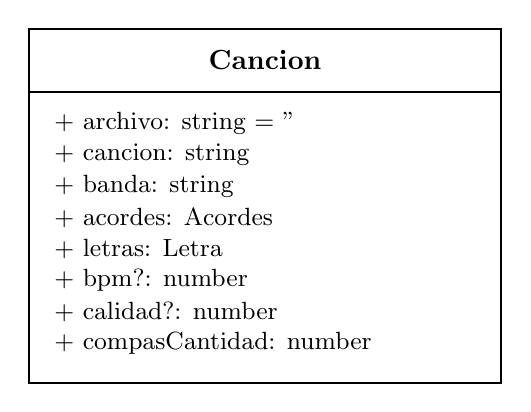
\begin{tikzpicture}
        % Dibujar el rectángulo de la clase
        \draw[thick] (0,0) rectangle (6,-4.5);
        % Línea para separar el nombre de la clase
        \draw[thick] (0,-0.8) -- (6,-0.8);
        % Nombre de la clase (centrado)
        \node at (3,-0.4) {\textbf{Cancion}};
        % Atributos
        \node[anchor=west, font=\small] at (0.2,-1.2) {+ archivo: string = ''};
        \node[anchor=west, font=\small] at (0.2,-1.6) {+ cancion: string};
        \node[anchor=west, font=\small] at (0.2,-2.0) {+ banda: string};
        \node[anchor=west, font=\small] at (0.2,-2.4) {+ acordes: Acordes};
        \node[anchor=west, font=\small] at (0.2,-2.8) {+ letras: Letra};
        \node[anchor=west, font=\small] at (0.2,-3.2) {+ bpm?: number};
        \node[anchor=west, font=\small] at (0.2,-3.6) {+ calidad?: number};
        \node[anchor=west, font=\small] at (0.2,-4.0) {+ compasCantidad: number};
    \end{tikzpicture}
    \caption{Diagrama de Clases de Cancion}
    \label{fig:diagrama-clase-cancion}
\end{figure}


[DIAGRAMA CANCION]


\paragraph{Relaciones entre Componentes}

\begin{itemize}
    \item El \textbf{Motor de Renderizado} consulta al \textbf{Gestor de Canciones} para obtener el contenido y al \textbf{Gestor de Configuración} para las preferencias de visualización.
    
    \item El \textbf{Motor de Sincronización} notifica al \textbf{Motor de Reproducción} sobre cambios en el compás y éste actualiza el \textbf{Motor de Renderizado}.
    
    \item El \textbf{Gestor de Sesiones} coordina con el \textbf{Motor de Sincronización} para mantener el estado compartido entre dispositivos.
    
    \item El \textbf{Gestor de Persistencia} provee datos tanto al \textbf{Gestor de Canciones} como al \textbf{Gestor de Usuarios}.
\end{itemize}

% TODO: Agregar diagrama de componentes UML mostrando las relaciones entre los componentes lógicos
% \begin{figure}[h]
%     \centering
%     \includegraphics[width=\textwidth]{imagenes/diagrama-componentes-logicos.png}
%     \caption{Diagrama de componentes lógicos del sistema El Fogón}
%     \label{fig:componentes-logicos}
% \end{figure}
